\chapter{Validation and additional features of the code}\label{ch07_validation}

The repository that handled the numerics in the previous chapter is called
\textit{ActiveDDFT}. I wrote this package to solve active DDFT
equations using pseudospectral collocation for various interactions and external
potentials.  In this chapter, I focus on additional features and validation of
the repository. First, I found the passive isotropic-nematic
(IN) transition which validates the code. Next, I studied the effects of
course-graining, finite-size, and concentration dependent diffusion for the hard
needle system. Finally, I present the temporal evolution of the density profile
for noninteracting particles in a harmonic well. I look at this particular
system because there is an analytic solution~\cite{doi_theory_88}, and it was
used in the microscopic binding model in our paper~\cite{maguire_design_18}. 

%%%%%%%%%%%%%%%%%%%%%%%%%%%%%%%%%%%%%%%%%%%%%%%%%%%%%%%%%%%%%%%%%%%%%%%
\section{Isotropic-nematic transition and numerical analysis}
% figure 4
\begin{figure}[!ht]
	\centering
  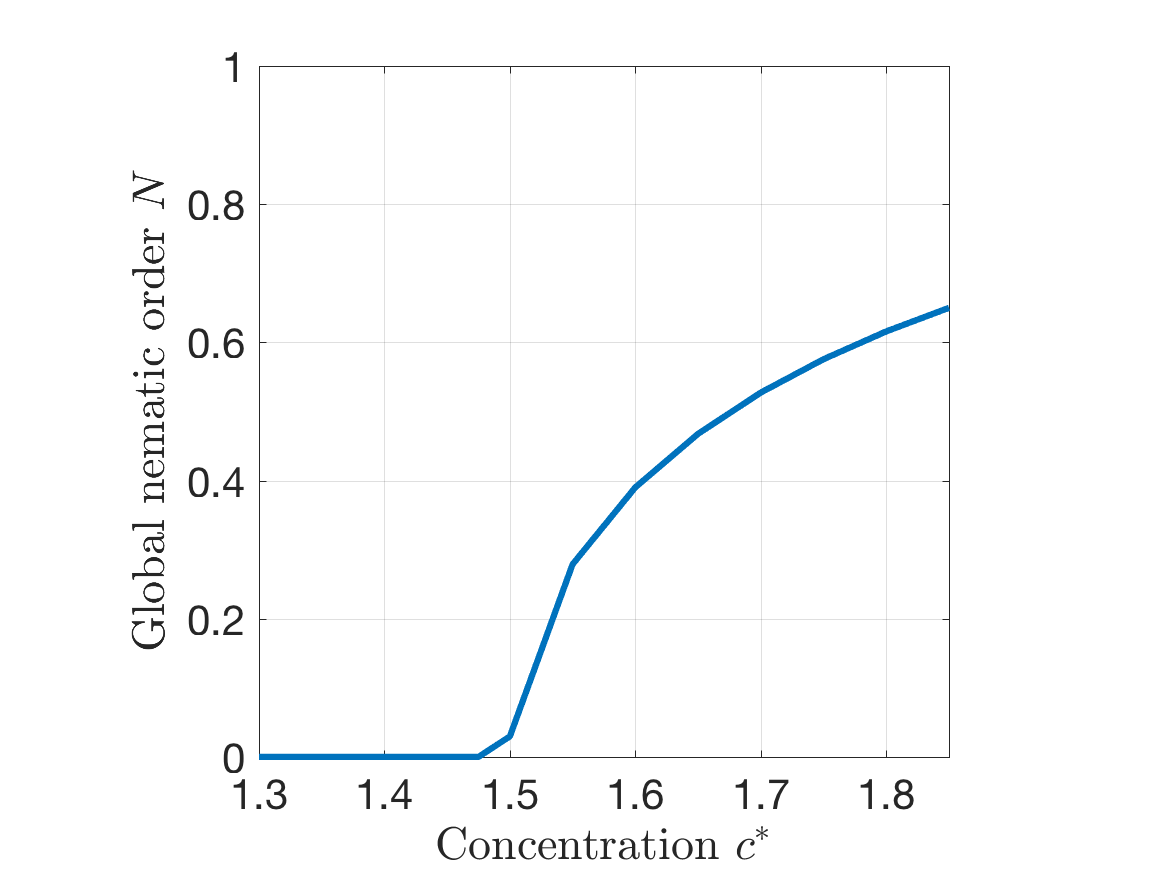
\includegraphics[width=0.50\textwidth]{figs/ch05_valid/in_trans.png}
  \caption[IN transition]
  {Nematic order as a function of concentration in the absence of driving.  The
    isotropic-nematic transition occurs at $c^* = 1.5$. The global nematic order
    parameter magnitude is the average of the local nematic order
    $N=\ev{N(x,y)}$. The system was homogeneous at all
    concentration.}\label{fig:in_trans}
\end{figure}
% figure

To validate the code, we studied the isotropic-nematic transition for passive
hard needles. The IN transition is second order and occurs at $c^*=1.5$ in
2D~\cite{kayser_bifurcation_78}. We measured the steady state global nematic
order parameter magnitude, $N = \ev{N(x,y)}$, as a function of
concentration~\figrefp{fig:in_trans}.  We found that a homogeneous isotropic is
stable for $c^*<1.5$.  At higher concentrations $c^*>1.5$, a homogeneous nematic
is stable. Reproducing equilibrium results validates our model.

%%%%%%%%%%%%%%%%%%%%%%%%%%%%%%%%%%%%%%%%%%%%%%%%%%%%%%%%%%%%%%%%%%%%%
\section{Concentration dependent diffusion}
% figure
\begin{figure}[!ht]
	\centering
  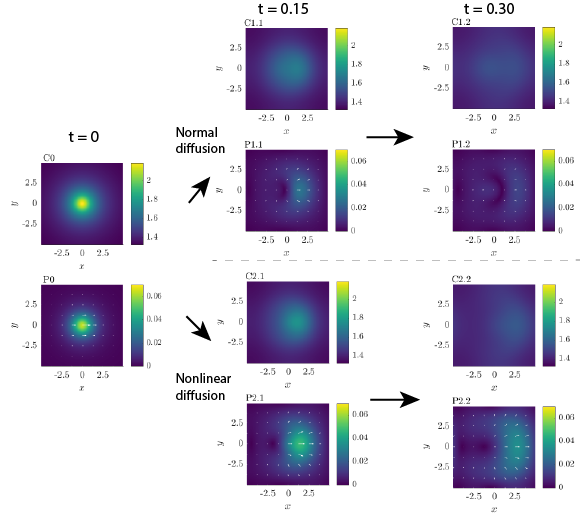
\includegraphics[width=0.85\textwidth]{figs/ch05_valid/nl_diff_break.png}
  \caption[Concentraion dependent diffusion (small flock perturbation)]
  {The nonlinear concentration dependent diffusion effects on a small
    amplitude Lorentzian perturbation flock state ($c^*=1.45$ and $\pe = 10$).
    The concentration (C*) and polar order (P*) are shown at different times for
    normal diffusion (top) and nonlinear diffusion with $C_{\perp,r} = 0.1$
    (bottom). Time progresses from left to right, and both cases start with the
    same initial condition. The titles refer to: CO/P0 concentration/polar order
    at $t=0$, C1.1/P1.1 concentration/polar order for normal diffusion at
    $t=0.15$, C2.1/P2.1 concentration/polar
    order for nonlinear diffusion at $t=0.15$, C1.2/P1.2 concentration/polar
    order for normal diffusion at $t=0.30$, C2.2/P2.2 concentration/polar
    order for nonlinear diffusion at $t=0.30$. The flock dissipated faster with
    normal diffusion. The final state for both systems was a homogeneous
    isotropic.}\label{fig:nl_diff_break}
  % fD = 10
  % bc = 1.45
  % particleMaster.nlDiff = {'aniso', 'rods', 0/0.1, [1 1]}; 
  % rhoInitMaster.intCond = {'iso'};
  % rhoInitMaster.perturb = { {'lorenz', 4, 1, 0, 1, 0, 1, 0} };
\end{figure}
% figure

% figure
\begin{figure}[!ht]
	\centering
  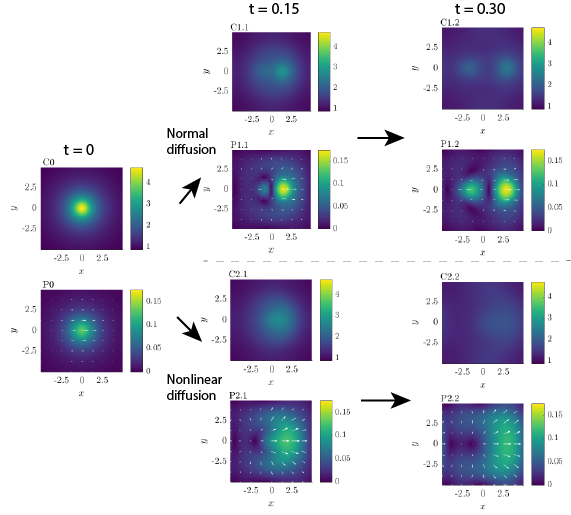
\includegraphics[width=0.85\textwidth]{figs/ch05_valid/nl_diff_back.png}
  \caption[Concentraion dependent diffusion (large flock perturbation)]
  {The nonlinear concentration dependent diffusion effects on a large
    amplitude Lorentzian perturbation flock state ($c^*=1.45$ and $\pe = 10$).
    The concentration (C*) and polar order (P*) are shown at different times for
    normal diffusion (top) and nonlinear diffusion with $C_{\perp,r} = 0.1$
    (bottom). Time progresses from left to right, and both cases start with the
    same initial condition. The titles refer to: CO/P0 concentration/polar order
    at $t=0$, C1.1/P1.1 concentration/polar order for normal diffusion at
    $t=0.15$, C2.1/P2.1 concentration/polar order for nonlinear diffusion at
    $t=0.15$, C1.2/P1.2 concentration/polar order for normal diffusion at
    $t=0.30$, C2.2/P2.2 concentration/polar order for nonlinear diffusion at
    $t=0.30$. For nonlinear diffusion, the flock slowly spread out as it
    traveled. For normal diffusion, there was an additional flock propagating in
    the opposite direction of the initial polar order. The final state for both
    systems was a homogeneous isotropic.}\label{fig:nl_diff_back}
  % fD = 10
  % bc = 1.45
  % particleMaster.nlDiff = {'aniso', 'rods', 0/0.1, [1 1]}; 
  % rhoInitMaster.intCond = {'iso'};
  % rhoInitMaster.perturb = { {'lorenz', 32, 1, 0, 1, 0, 1, 0} };
\end{figure}
% figure


In the previous chapter, we took the dilute limit for the diffusion
coefficients. However, diffusion can be slowed by crowding effects. For thin
rods~\cite{doi_theory_88,frenkel_molecular_81, frenkel_molecular_83,
  liverpool_instabilities_03}, this effect is dominant in the perpendicular 
%
\begin{equation}~\label{eqn:dnl_perp}
  D_{\perp}(\bm{r}) \simeq \frac{D^0_{\perp} } {{[ 1 + c(\bm{r})/C_{\perp} ]}^2 } ,
\end{equation}
%
and rotational
%
\begin{equation}~\label{eqn:dnl_r}
  D_{r}(\bm{r}) \simeq \frac{D^0_r}{{[ 1 + c(\bm{r})/C_{r} ]}^2},
\end{equation}
%
diffusion coefficients where $C_{r}$, $C_{\perp}$ are constants of order 1 and
$c(\bm{r})$ is the local concentration. The parallel component is essentially
unaffected by crowding~\cite{liverpool_instabilities_03}, and its scaling with
concentration is given elsewhere~\cite{frenkel_molecular_81,
  frenkel_molecular_83}. 

We studied the effects of nonlinear concentration dependent diffusion on
constructed flock states. Our initial state was a homogeneous
isotropic with an additive Lorentzian perturbation. We set the width of the
Lorentzian to be $1$ in $x$, $y$, and $\phi$.  We investigated the effects of
diffusion for small \figrefp{fig:nl_diff_break} and large ($4$ times the
magnitude of the small) perturbations \figrefp{fig:nl_diff_back}. We show the concentration and polar order for normal diffusion (top panel) and
nonlinear diffusion (bottom panel). Both cases start with the same initial
condition, and time increases from left to right. For all simulations, we set
$c^*=1.45$ and $\pe = 10$. We exaggerated the effects of differing diffusion
coefficients by setting $C_{r}, C_{\perp} = 0.1$ in the nonlinear case. Normal
diffusion refers to the dilute limit.

For small perturbations \figrefp{fig:nl_diff_break}, the flock with normal
diffusion disintegrates faster than the nonlinear case. The flock breaks up
because rods on the edge quickly rotate away from the center and leave the
cluster. Since the rotational diffusion is smaller for the nonlinear diffusion,
this effect is minimized, and the flock is more stable. 

For larger perturbations \figrefp{fig:nl_diff_back}, the nonlinear case behaves
qualitatively the same as for small perturbations. However, the normal
diffusion system behaves differently; two counterpropagating
flocks form. This is because the center of the flock is at high
concentration and, therefore, wants to form a nematic. Since the rods are free
to rotate even at high density (which is not physical), we get a nematic in the
center of the flock. Thus, we get two counterpropagating flocks along the
nematic director. These flock results provided us with evidence that the
functional was not encapsulating the physics seen in simulations. In jammed
flocks, rods should not be free to rotate. Even with a modified diffusion
coefficient, there was no flocking state in DDFT\@.

% figure 4
\begin{figure}[!b]
	\centering
  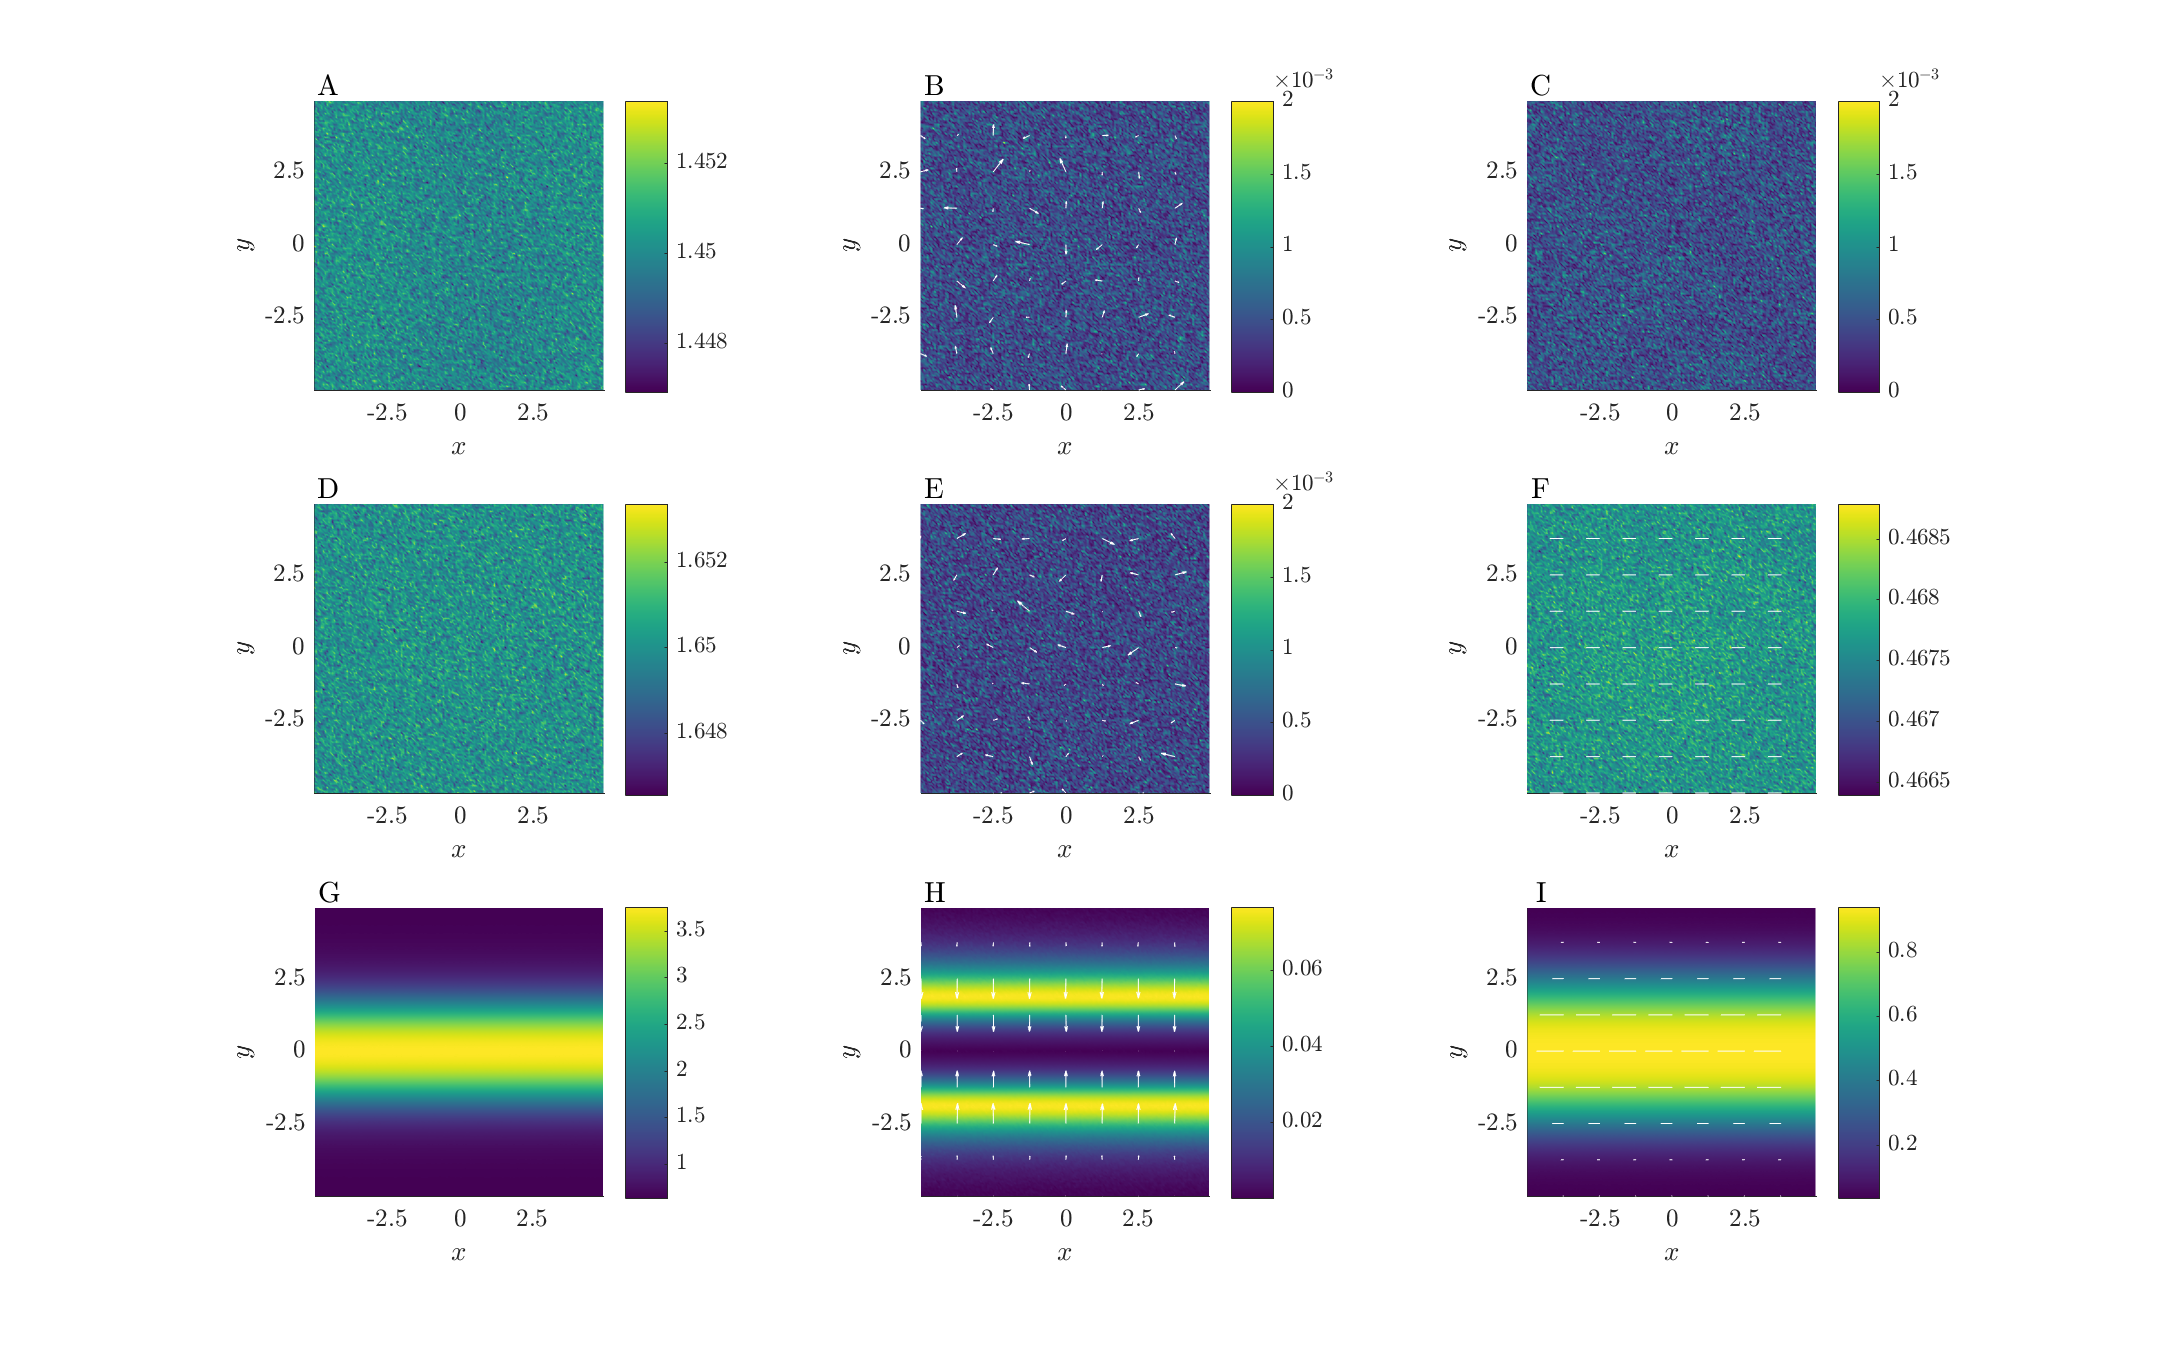
\includegraphics[width=1.00\textwidth]{figs/ch05_valid/noise_compare.png}
  \caption[Course-graining]
  {Snapshots of the concentration and order parameters showing the effects of
    course-graining on the three active needle phases. For all panels, the noise
    strength is $\Delta = 1$. Top
    panel: (A) concentration, (B) polar order, and (C) nematic order for a
    homogeneous isotropic with $c^* = 1.45$ and $\pe = 0$. Middle panel:
    (D) concentration, (E) polar order, and (F) nematic  order for a
    homogeneous nematic with $c^* = 1.65$ and $\pe = 0$. Bottom panel:
    (G) concentration, (H) polar order, and (I) nematic order for a
    band state with $c^* = 1.65$ and $\pe = 30$.}\label{fig:noise_compare}
\end{figure}
% figure

%%%%%%%%%%%%%%%%%%%%%%%%%%%%%%%%%%%%%%%%%%%%%%%%%%%%%%%%%%%%%%%%%%%%%
\section{Effects of course-graining}

The dynamical density functional theory equation \eqnrefp{eqn:ddft_intro}
describes the temporal evolution of the ensemble averaged density. Typically in
simulation or experiment, a course-grained density $\bar{\rho}$ is measured by
averaging the microscopic density over some time or spatial
window~\cite{archer_dynamical_04a}. The dynamics of the course-grained density
are given by~\cite{dean_langevin_96, archer_dynamical_04a,
  mishra_fluctuations_10}
%
\begin{equation}\label{eqn:course_grain}
  \frac{\partial \bar{\rho} ( \bm{r},\hat{\bm{u}},t )}{\partial t} = 
  \boldsymbol{\nabla} \cdot \left[ \bar{\rho}( \bm{r},\hat{\bm{u}},t )
    \boldsymbol{\nabla} \frac{\delta \mathcal{F} 
      \left[ \bar{\rho}( \bm{r}, \hat{\bm{u}},t ) \right]}
    {\delta \bar{\rho}( \bm{r},\hat{\bm{u}},t )}
    + \cdot \zeta^{-1} \sqrt{\bar{\rho}( \bm{r},\hat{\bm{u}},t )}
    \bm{\xi}(\bm{r},\hat{\bm{u}},t)\right],
\end{equation}
%
where $\bm{\xi}$ is a random vector field with properties
%
\begin{gather}
  \langle \boldsymbol{\xi}(\bm{r},\hat{\bm{u}},t) \rangle = 0 \\
  \langle \xi^l(\bm{r},\hat{\bm{u}},t) \xi^m (\bm{r}',\hat{\bm{u}}',t') \rangle 
  = 2 k_B T \zeta
  \Delta \delta_{lm} \delta( \bm{r} - \bm{r}' ) \delta( \bm{\hat{u}} -
  \bm{\hat{u}}' ) \delta( t - t' ),
\end{gather}
%
where $\Delta$ is the effective strength of the
noise~\cite{mishra_fluctuations_10}.  There has been a bit of confusion in the
literature in regards to this noise term (clarified in
\cref{archer_dynamical_04a}). Random fluctuations are inherent to the dynamics
of the microscopic density operator, and therefore, its evolution is stochastic.
The ensemble averaged density, however, is an average over all noise
realizations and therefore, deterministic. Noise is the source of diffusion. The course-grained density is
an incomplete averaging of all possible noise fluctuations. Thus, its evolution
is stochastic~\cite{archer_dynamical_04a}. The term noise strength, as mentioned
in~\cite{mishra_fluctuations_10}, is misleading.  Including a noise term
in~\ref{eqn:course_grain} is not a more rigorous consideration of noise; it
means that we are dealing with a course-grained density and not the ensemble
averaged density. Furthermore, this noise strength is a measure of the
degree of course-graining
% 
\begin{equation}
  \Delta = \frac{\tau_0}{\tau},
\end{equation}
%
where $\tau_0$ is a some characteristic microscopic time scale and $\tau$ the
characteristic course-graining time scale~\cite{archer_dynamical_04a}. Note that
in the long time average limit ($\tau \gg \tau_0$) the noise term goes to zero,
and we recover the DDFT \eqnref{eqn:ddft_intro} from \eqnref{eqn:course_grain}.

I studied the effects of course-graining on the three steady state phases of
the active needle system: isotropic, nematic, and band
\figrefp{fig:noise_compare}. Note that the color scales were intentionally set
to different limits to show the fluctuations from noise
\eqnrefp{eqn:course_grain}. For all cases, the fluctuations are constantly
varying with time. However, the general structure of the three states in
unaltered. 

\subsection{Comparing simulation to DDFT}
To compare DDFT and simulations, one must average over many
simulations~\cite{dzubiella_meanfield_03, archer_dynamical_05,
  archer_interplay_11}. Each simulation must begin with similar initial
conditions, \textit{i.e.}, the initial positions of all particles are sampled
from the initial density $\rho(\bm{r}, t=0)$ for each simulation. The ensemble
averaged density at a given time $t$ is the average over all microscopic
densities from simulations at $t$. 

Given how rapidly the density fluctuations traveled in the active needle
simulations, one could image that averaging over many simulations could smear
out the flocking dynamics in DDFT\@.  For example, consider running many
simulations of a single flock. The flock travels as a collective structure for a
long time in any given simulation. However, on average, the density would spread
out because the flock has equal probably to turn left or right. With many
flocks, averaging over several simulations may cause the density to appear
homogeneous but with large fluctuations.  We believe this effect contributed to
the absence of flocking in DDFT\@. However, as mentioned in the previous
chapter, there is physics the functional cannot capture. The functional
approximation is probably the most significant reason why flocking does not
occur in the DDFT calculations.

It is natural to wonder why DDFT can show
crystallization~\cite{choudhary_ddft_11,kahl_classical_09,archer_quasicrystalline_13}
if a homogeneous liquid is equally likely to crystallize at any
position, \textit{i.e.}, the free energy minimum is invariant under
translations of the entire crystal. In DDFT, a crystal forms in a deterministic
location because fluctuations in the initial
conditions~\cite{malijevsky_sedimentation_13} (due to density perturbations) or
a hard wall boundary~\cite{archer_quasicrystalline_13} break the symmetry.
Equilibrium phase transitions are different from the dynamical phases because in
some dynamical phases (like flocking) the jammed structures are not static.

%%%%%%%%%%%%%%%%%%%%%%%%%%%%%%%%%%%%%%%%%%%%%%%%%%%%%%%%%%%%%%%%%%%%%
\section{Finite-size effects}
% figure
\begin{figure}[!ht]
	\centering
  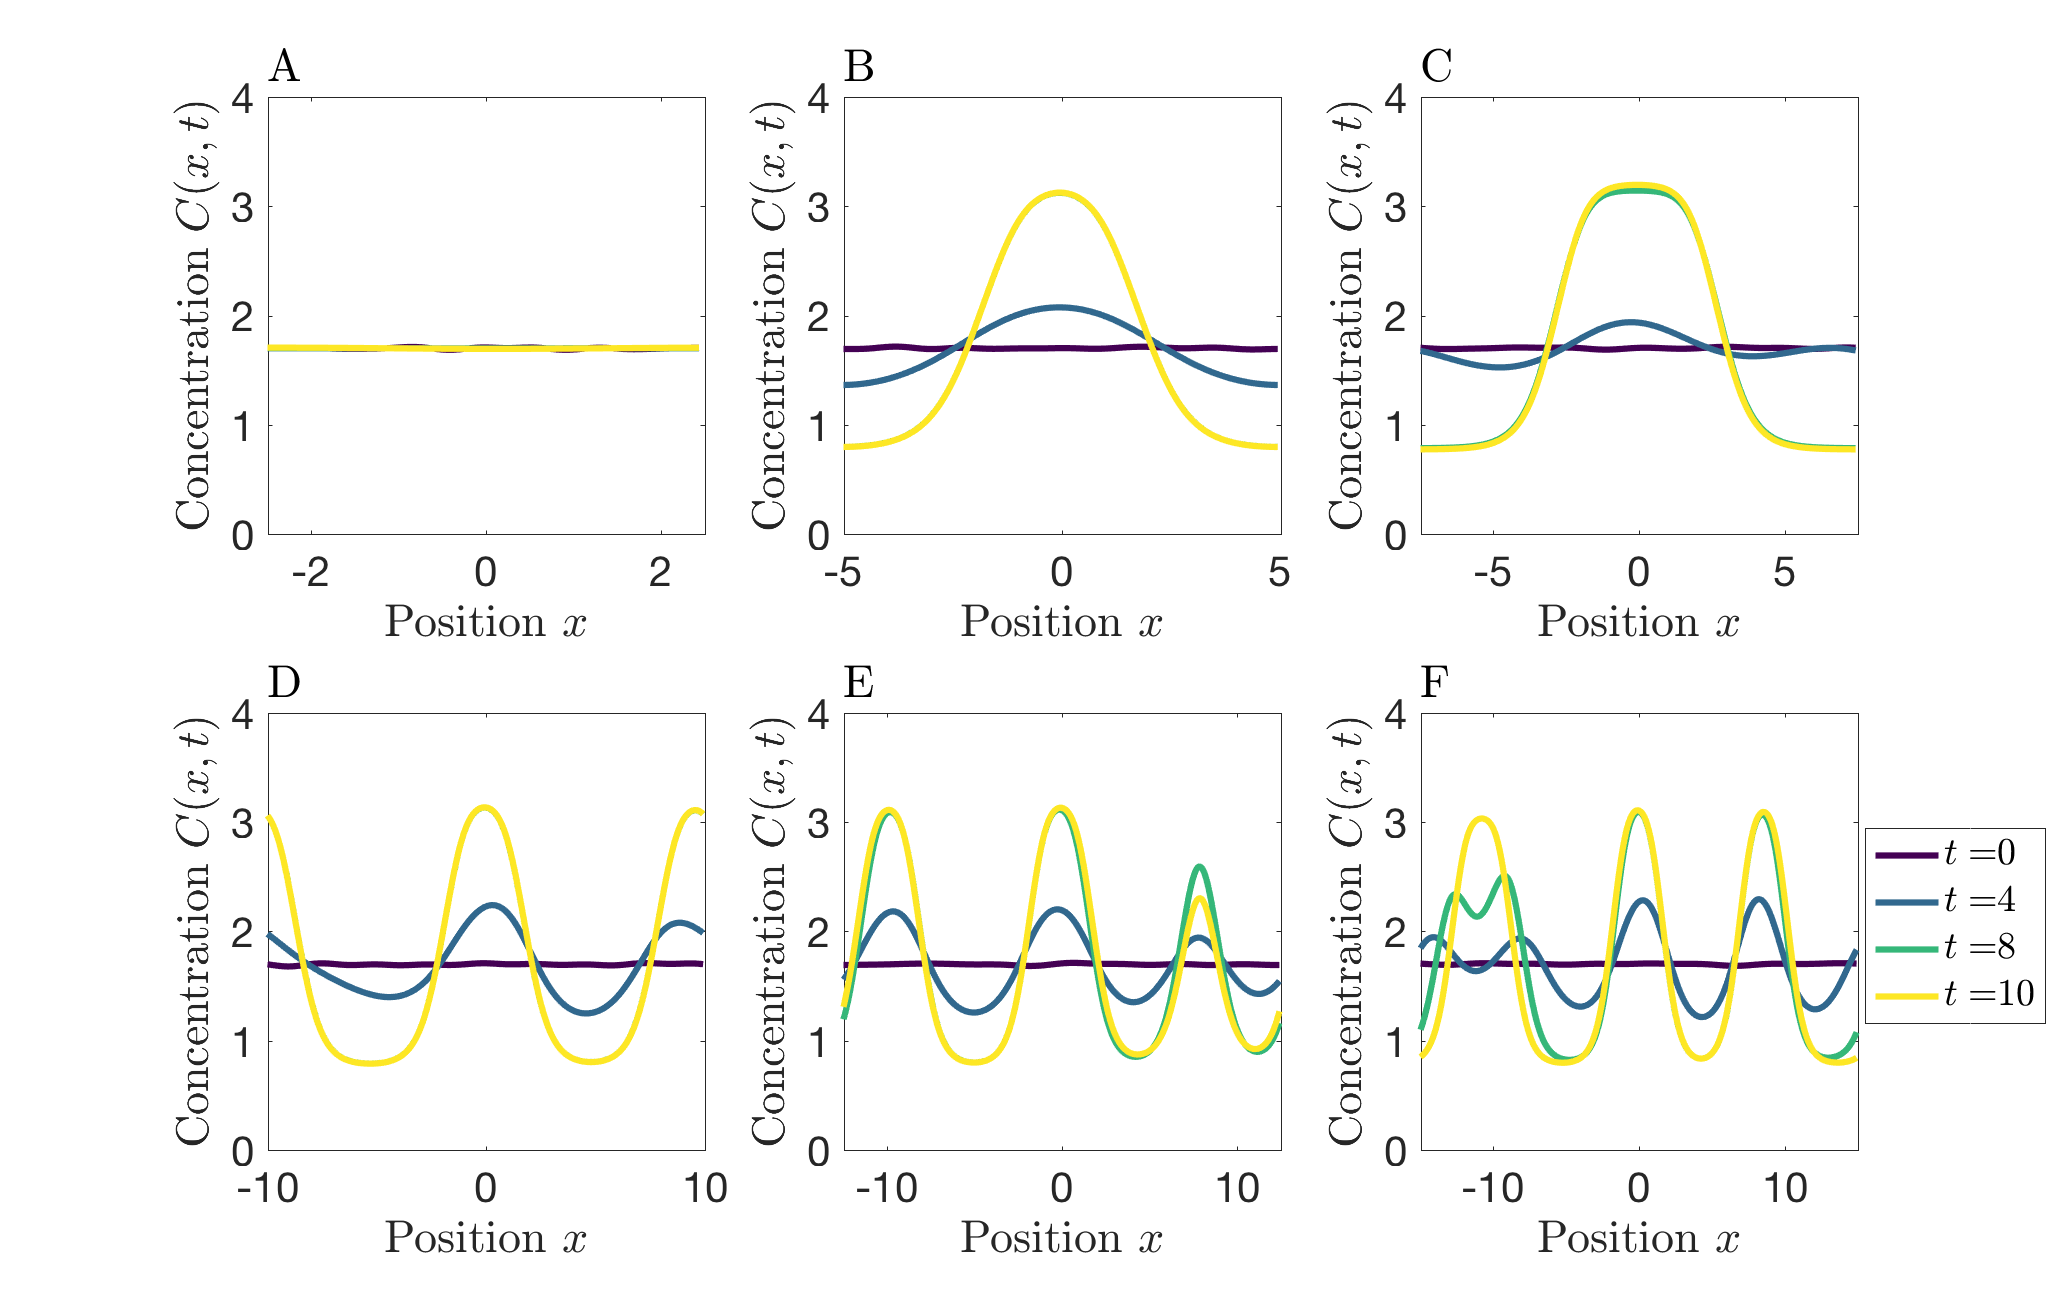
\includegraphics[width=1.00\textwidth]{figs/ch05_valid/box_size_compare_eq.png}
  \caption[Finite-size effects: homogeneous nematic initial condition]
  {The effects of box size on the band state with $c^*=1.70$ and $\pe = 20$. 
  The concentration along
  the inhomogeneous direction is plotted as function of position
  at various times (indicated by color) for: 
  (A) $L_{\tx{box}}=5$, (B) $L_{\tx{box}}=10$, 
  (C) $L_{\tx{box}}=15$, (D) $L_{\tx{box}}=20$, (E)
  $L_{\tx{box}}=25$, (F) $L_{\tx{box}}=30$. 
  The initial condition was a homogeneous nematic with
  random perturbations. The concentration was
  shifted in the plots so that the highest peak is at $x=0$.}\label{fig:box_size_eq}
\end{figure}
% figure
% figure
\begin{figure}[!ht]
	\centering
  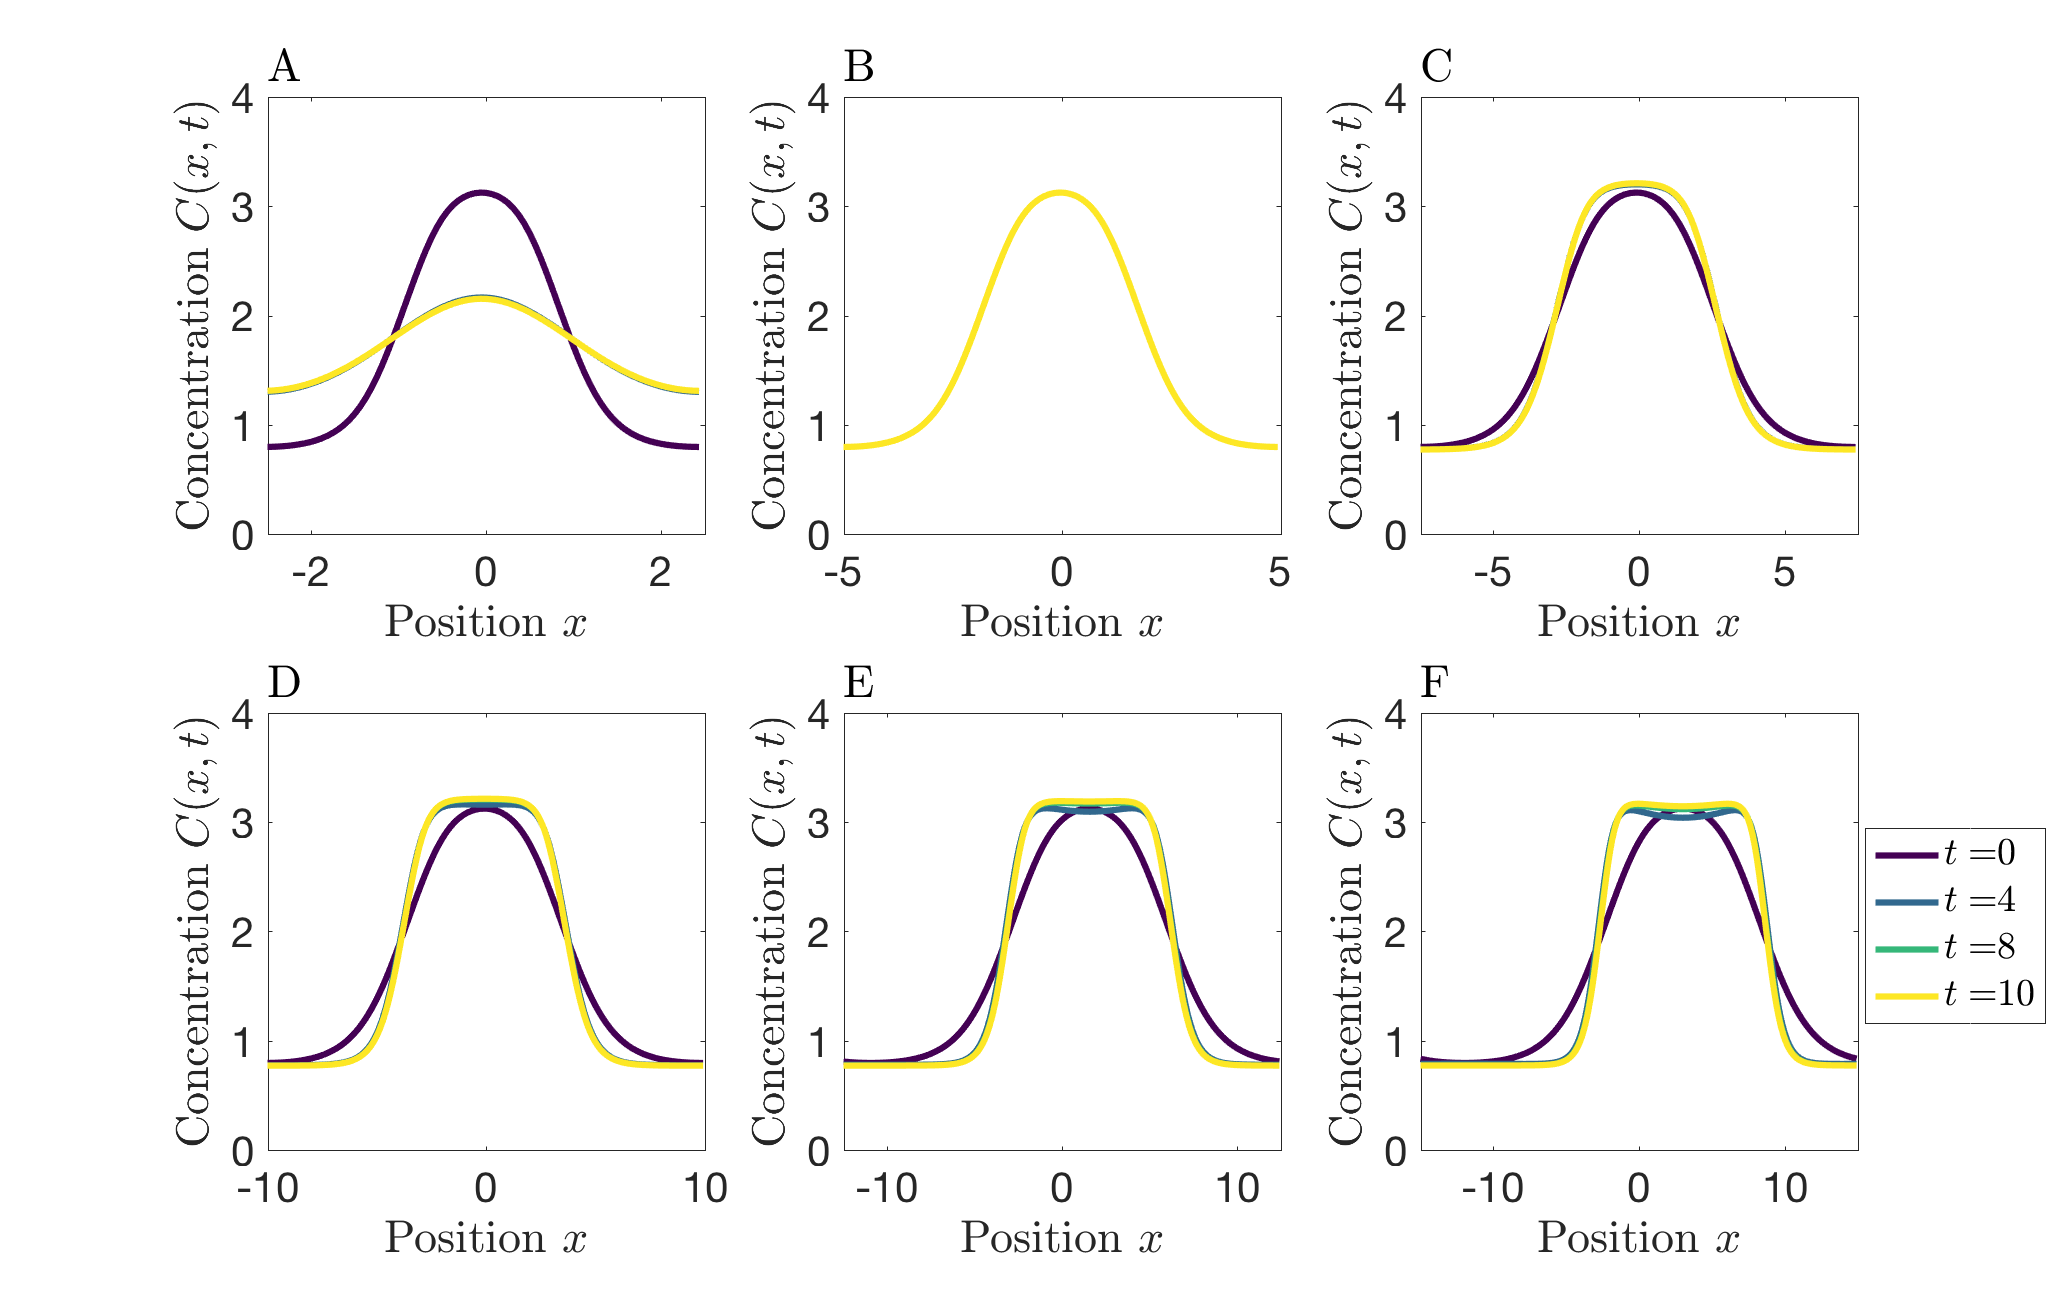
\includegraphics[width=1.00\textwidth]{figs/ch05_valid/box_size_compare_band.png}
  \caption[Finite-size effects: band initial condition]
  {The effects of box size on the band state with $c^*=1.70$ and $\pe = 20$. 
  The concentration along
  the inhomogeneous direction is plotted as function of position
  at various times (indicated by color) for: 
  (A) $L_{\tx{box}}=5$, (B) $L_{\tx{box}}=10$, (C) $L_{\tx{box}}=15$, (D) $L_{\tx{box}}=20$, (E)
  $L_{\tx{box}}=25$, (F) $L_{\tx{box}}=30$. The initial condition was the steady state
  solution for a box size $L_{\tx{box}}=10$.The concentration was
  shifted in the plots so that the highest peak is at $x=0$.}\label{fig:box_size_band}
\end{figure}
% figure

We studied the effects of box size on the active needle band state. We varied
the box in the direction of inhomogeneity while keeping the other dimension
fixed. We looked at two initial conditions: a homogeneous nematic
\figrefp{fig:box_size_eq} and band state \figrefp{fig:box_size_band}. For both,
the concentration was $c^* = 1.7$, and driving was $\pe =20$.  The band state
initial condition was the steady state solution for a box size $L_{\tx{box}}=10$
($c^* = 1.7$, $\pe =20$). Note, the maximum concentration was centered at $x=0$
for all plots. For both initial conditions, box size played a role. For the
nematic initial condition \figrefp{fig:box_size_eq}, the band state did not form
at the smallest box size $L_{\tx{box}}=5$ during the run; however, a single band
formed at later times (results not shown).  For $L_{\tx{box}}=10$ and
$L_{\tx{box}}=15$, a single band formed and was stable. Multiple bands formed
for larger boxes.  Some bands were transient over the course of the
simulation, \textit{e.g.}, two separate peaks in $L_{\tx{box}}=30$ at $t=4$
combined by $t=10$. Note, these runs had not reached steady-state.  These
results show that multiple transient bands can form at larger box sizes. At
a later time ($t=20$) for $L_{\tx{box}} = 20$ and $L_{\tx{box}} =
25$, two bands were stable (results not shown), which suggests that multiple
bands are stable in larger boxes.

In \figref{fig:box_size_band}, we studied the stability of a single band. The
band shape changed with the box length. At larger box lengths, the band became
more step-like. There was no evidence that the single band was unstable. The
results in \figref{fig:box_size_eq} and \figref{fig:box_size_band} suggest that
the initial condition effects the number of bands. This differs from the
homogeneous nematic to band transition, which is independent of initial
condition.

%%%%%%%%%%%%%%%%%%%%%%%%%%%%%%%%%%%%%%%%%%%%%%%%%%%%%%%%%%%%%%%%%%%%%
\section{External potentials in DDFT}
% figure 4
\begin{figure}[!ht]
	\centering
  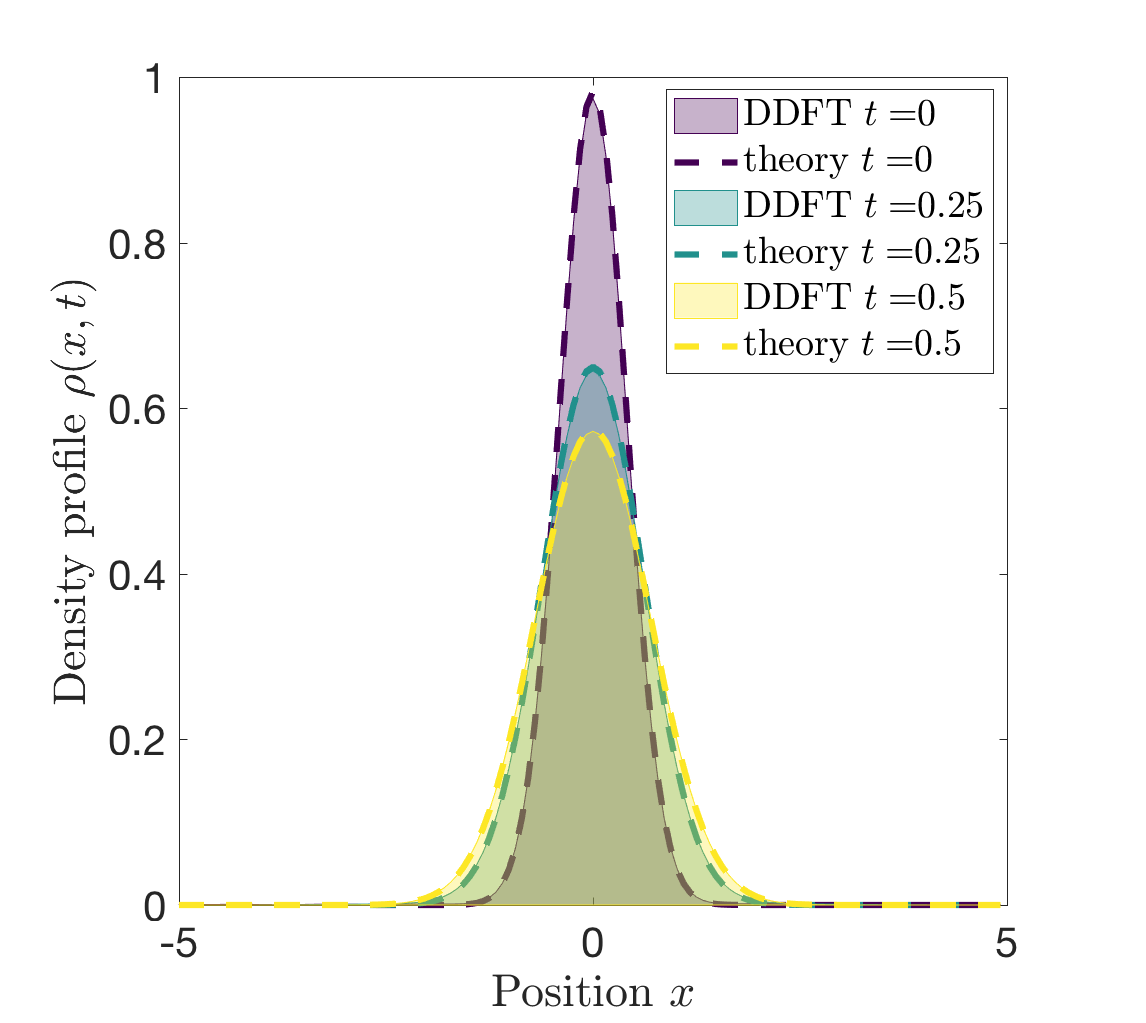
\includegraphics[width=0.50\textwidth]{figs/ch05_valid/external_pot_validation.png}
  \caption[External potential validation]
  {A comparison of the DDFT and analytic solution for noninteracting
    Brownian particles in a harmonic well. Time is indicated by color. The
  filled curve is the DDFT solution, and the dashed line is the analytic
  solution. The DDFT and analytic solution match at all times.}\label{fig:ext_pot}
\end{figure}
% figure

Up till now, we have not studied the effects of external potentials. Since the
free energy is separable, the effects of an external potential is additive in
DDFT~\cite{archer_dynamical_04}
%
\begin{align}
  \diff{\rho(\bm{r,\hat{\bm{u}},t})}{t} = 
  \bm{\nabla}  \cdot \zeta^{-1} \left[  
    k_B T \bm{\nabla} \rho(\bm{r},\hat{\bm{u}},t) 
    + \rho(\bm{r},\hat{\bm{u}},t) \bm{\nabla}
    \frac{\delta \mathcal{F}^{\tx{ex}} \left[ \rho \right]}
  {\delta \rho(\bm{r},\hat{\bm{u}}, t ) } 
  +\rho(\bm{r},\hat{\bm{u}}, t )\bm{\nabla} V_{ext}(\bm{r}, \hat{\bm{u}}, t)
\right],
\end{align}
%
where $V_{\tx{ext}}$ is the external potential.  To validate the numerics, we
compared the numerical solution for noninteracting particles in a harmonic well
$V_{\tx{ext}} = \frac{1}{2}k x^2$ to the analytic solution~\cite{doi_theory_88}.
The equation of motion for the one-dimension case is
%
\begin{align}
  \label{eqn:harmonic}
  \diff{\rho(x, t)}{t} = 
  D \secdiff{\rho(x,t)}{x}   + 
  Dk\beta \diff{}{x} \left[ x \rho(x, t ) \right],
\end{align}
%
where $k$ is the spring constant and $\beta = 1/k_B T$. The analytic solution is 
%
\begin{equation}~\label{eqn:analytic_harm}
  \rho(x,t) = \frac{1}{\sqrt{2\pi \alpha(t)}}
e^{-\frac{x^2}{2 \alpha(t)}},
\end{equation}
%
where $ \alpha(t) = \frac{1}{\beta k}(1-e^{-2kD\beta t})$.
In \eqnref{eqn:analytic_harm}, the initial condition is a delta function centered
at $x=0$. To compare the DDFT to the analytic solution, we used the initial
condition
%
\begin{equation}
  \rho(x,t=0) = \frac{1}{\sqrt{2\pi \alpha(0.1)}}
e^{-\frac{x^2}{2 \alpha(0.1)}}.
\end{equation}
%
Using a Gaussian as an initial condition avoids numerical issues with sharply
peaked delta functions.  The comparison between the analytic and DDFT solution
with $D=1$ and $k=2$ is shown in \figref{fig:ext_pot}. The shaded curve is the
DDFT solution, the dashed line is the analytic solution, and the color indicates
the time. For the DDFT solution, we solved the system in 2D with the potential
along $x$ and took a slice along $P(x,y=0,t)$ (there was no variation along
$y$). Note, the analytic solution is for infinite boundaries while DDFT has
periodic boundaries. I selected a box size where boundary effects did not
influence the solution. We see excellent agreement between the numerics and
analytic solution. This test validates external potentials in the code. While
this case was a one-dimensional example, the code can handle potentials for up
to three dimensions.
